
\clearpage

\section{Una revisión al ADN}
El ácido desoxirribonucleico, conocido comúnmente como ADN debido a sus siglas, es una molécula compleja que se encuentra en todos los seres vivos y en algunos virus,tiene la información necesaria para construir y mantener un organismo, y sí el organismo lo quiere tiene la función de ser la unidad primaria de la herencia.\\

El objetivo de este capitulo es dar una breve introducción de como esta compuesto el ADN, su historia, su estrecha relación con la radiación junto con los efectos que puede generar el alterarlo, y los mecanismos asociados al ADN y a las células para reparar daños e impedir algún mal funcionamiento.\\


\subsection{Historia del ADN}
La epopeya del ADN tiene sus inicios en 1869 con un bioquímico llamado Friedrich Miescher, quien estaba interesado en la estructura química de las fascinantes unidades fundamentales de la vida conocidas como células.
Miescher viajaba todos los días a la clínica más cercana para tomar las vendas sucias, esto debido a que estaban recubiertas de pus (lo cual era una buena fuente de leucocitos), añadiendo álcali hizo que los núcleos se abrieran liberando sus componentes, de esta manera Miescher extrajo un componente(ADN), al que el nombro nucleína, realizando un análisis de esta nucleína mostró que era un ácido que contenía fósforo y por tanto no calificaba en en ninguno de los grupos conocidos en ese momento como carbohidratos y proteínas, este fue clasificado como un ácido nucleico y su relevancia biológica no fue descubierta hasta mucho tiempo después \cite{Susan}.\\

En 1928 Fredrick Griffith realizaba una investigación con neumococos, tenia dos tipos: el primero patógeno  fue cultivado en placas de petri conocido como S(smooth-suave) debido a su apariencia, el segúndo inofensivo y conocido como R(rough-áspero), Griffith descubrio que al añadir un extracto de los neumococos tipos S al tipo R, este ultimo podría heredar las propiedades del tipo S, este fenómeno recibió el nombre de principio de transformación e indicaba que el extracto contenía la molécula de la herencia.\\

Oswald Avery junto con MacLeod y McCarty demostraron que substancia efectiva en el experimento de Griffiths era la molécula de ADN y que a su vez, era el portador de genes en la célula, también es importante mencionar que Alfred Hershey y Martha Chase quienes confirmaron la conclusión en 1952 mediante experimentos con trazadores radioactivos\cite{Thormod}.\\

Es relevante mencionar otros aportes significativos: \\
1.Erwin Chargaff encontró una regularidad peculiar en los radios de las bases de los nucleótidos.\\
2.Sven Furger trabajo en la estructura de los componentes del ADN, encontró que la base plana(plano de la citosina) era perpendicular a la molécula de azúcar.\\
3.Rosalind Franklin logro distinguir dos tipos de ADN dependiendo de la hidratación y que ambos tenían estructura helicoidal mediante cristalográfia, véase figura ~\ref{fig:rf}.\\

\begin{figure}[htbp]
    \centering
    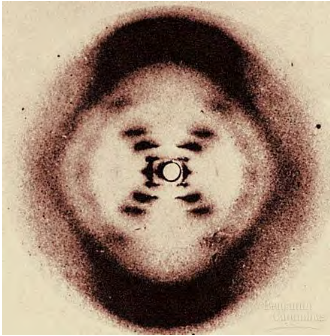
\includegraphics[width=0.5\linewidth]{./Figures/RF.png}
    \caption[Fotografía cristalográfica del ADN]{Fotografiá cristalográfica del ADN tomada por Rosalind Franklin en 1952}
    \label{fig:rf}
\end{figure}
El ultimo paso hacia la estructura del ADN fue llevado acabo por James Watson y Francis Crick en el laboratorio de Cavendish en francia, juntos trabajaron en diferentes modelos de la molécula de ADN , en 1953 publicaron un articulo en la prestigiosa revista Nature titulado: "molécular Structure of Nucleid Acids", el articulo solo tenia una pagina, pero era de un impacto significativo debido al modelo de ADN que contenía, un modelo de doble hélice(figura ~\ref{fig:jw}), ademas de esto, sugerían que el emparejamiento  especifico que habían postulado intuía un posible mecanismo para copiar material genético.
\begin{figure}[htbp]
    \centering
    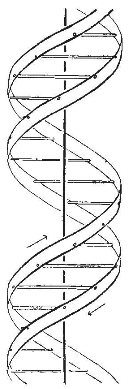
\includegraphics[width=0.15\linewidth]{./Figures/DNA1.png}
    \caption[Diagrama esquemático del ADN]{Diagrama esquemático del ADN publicado por Watson y Crick en 1953, imagen tomada de \cite{jwfc}.}
    \label{fig:jw}
\end{figure}
\subsection{Estructura del ADN}
el ADN es una molécula compuesta por dos largas cadenas, estas cadenas están formadas de múltiples
nucleótidos y cada
nucleótido esta compuesto por una base una molécula azúcar y un grupo fosfato.\\
El código genético del ADN esta representado por grupos de cuatro tipos de base con secuencias especificas. En el ADN, el azúcar es desoxirribosa, y esta unida a un grupo fosfato,  la base puede ser adenina (A), citosina (C), guanina (G), o timina (T), los nucleótidos están unidos covalentemente en una cadena mediante azúcar y fosfatos, y forman una estructura en forma de cadena alternando azúcar-fosfato-azúcar-fosfato. La estructura tridimensional del DNA(Doble hélice) surge de las características químicas y estructurales de las dos cadenas de
nucleótidos. Debido a que las dos cadenas se sostienen juntar debido a los enlaces de hidrógenos entre las base (A y T; G y C), todas las bases se encuentran en el lado interna de las hélices mientas que los grupos azúcar fosfato en la parte exterior\cite{rescells}.

\subsubsection{Daño inducido por radiación al ADN}

 Cualquier forma de radiación tiene el potencial de interactuar con estructuras claves como lo son los átomos para generar ionización, una vez suceda esto se inician eventos en cadena que llevan a cambios biológicos, estos efectos biológicos presentes en algún ser vivo debido a la radiación son relacionados a daños en el ADN.\\
 Esto se conoce como  acción directa de la radiación, y es el proceso dominante para radiación con gran cantidad de transferencia lineal de energía (LET) tales como partículas $\alpha$ o neutrones\cite{rescells}.\\

Por otro lado se tiene la acción indirecta de la radiación, este tipo de daño se ha demostrado mediante múltiples investigaciones\cite{willmari}, la radiación puede interactuar con los átomos de moléculas de una célula(particularmente con agua) para producir radicales libres, los cuales se pueden difundir lo suficientemente lejos para interactuar con objetivos críticos y causar daños, los radicales libres tienen electrones desapareados lo que causa gran reactividad química. La mayoría de la energía  depositada en células es inicialmente absorbida por el componente principal de las células, el agua, esto conlleva a una producción rápida de oxidantes y reductores de radicales hidroxilo reactivos. Los radicales hidroxilo pueden difundirse lo suficiente para interactuar con el ADN y causar daños. Afortunadamente, algunos sistemas defensivos o respuestas en las células pueden proteger a las células de los daños\cite{rescells}.\\

Evidencia acumulada en estudios radiológicos \cite{Franklin},\cite{rescells},  sugieren al ADN como el  objetivo sensible a la radiación. Esto se traduce en lesiones o modificaciones a genes y cromosomas, entender estos cambios son fundamentales para investigar y comprender la carcinogénesis, la muerte celular inducida por la radiación, y la transformación celular.\\


\paragraph{Rompimientos simples}
Un rompimiento simple es un rompimiento en un enlace peptídico, es decir azúcar fosfato, este daño es usualmente fácil de reparar, y en experimentos  se ha demostrado que aproximadamente el 90\% de los rompimientos simples son reparados en el curso de una hora a una temperatura de $37^{\circ} C$ \cite{Thormod}

\paragraph{Rompimientos dobles}

Este tipo de daño involucra las dos cadenas  del ADN, Si el enlace peptídico se rompe a cada lado dentro de una distancia de unos cuantos pares base se presentara un rompimiento doble, estos suelen estar relacionados con muerte celular y daño a los cromosomas.\\
Los rompimientos dobles son posibles de reparar, sin embargo, es mucho más difícil de reparar que un rompimiento simple,
la molécula de ADN contiene proteínas que suportan la estructura y previene que las piezas se caigan incluso cuando un rompimiento ocurre en ambas cadenas del ADN, de hecho, existen un numero de mecanismos que organismos complejos(como los humanos) han evolucionado para reparar los rompimientos dobles\cite{Thormod}.

\begin{figure}[htbp]
    \centering
    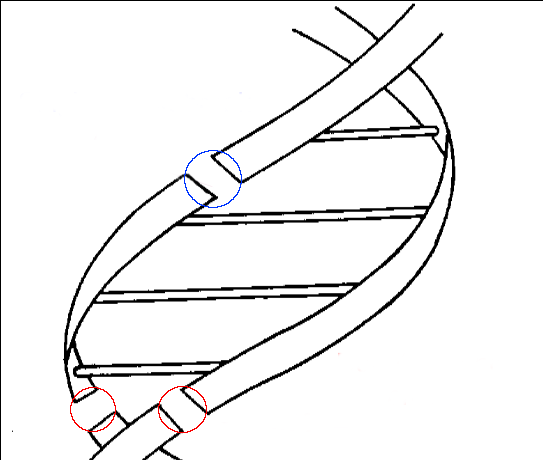
\includegraphics[width=0.5\linewidth]{./Figures/esbdb.png}
    \caption[Esquema rompimientos simples y dobles]{Rompimiento doble en rojo y rompimiento simple en azul, adaptada de \cite{Thormod}}
    \label{fig:esbdb}
\end{figure}


\paragraph{Daño base}

Como resultado de un fallo al reparar o de una falta de reparación, el codon(una secuencia de tres nucleótidos) alterado puede insertar un aminoácido incorrecto en la proteína y a su vez, la proteína modificada podría no funcionar correctamente, Si una base es alterada, la información puede cambiar o perderse,es conveniente mencionar que el daño a la base es uno de los puntos iniciales para la mutación. \\
Experimentos indican que la sensibilidad a la radiación varia de una base a otra. Después de una ionización inicial, rápidas organizaciones electrónicas toman lugar con el resultado de que el daño es transportado a ciertas regiones de la macromolécula (La guanina es particularmente sensible)\cite{Thormod}.

\paragraph{Dimeridos de pirimidina}

Se conoce a dímeros de pirimidina cuando dos bases adyacentes, (T y T, para la figura ~\ref{fig:dbdi})en la misma cadena se han alterado (sea químicamente o por cualquier otro motivo),  sucede entonces  que se necesita una de las cadenas para replicar la cadena siguiente, como efecto cuando ambas cadenas están dañadas en el mismo sitio no hay manera de que esto se lleve acabo.

\begin{figure}[htbp]
    \centering
    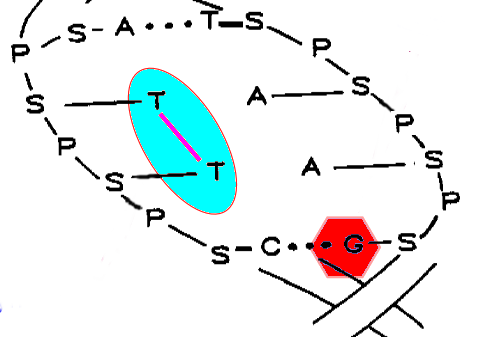
\includegraphics[width=0.5\linewidth]{./Figures/base-piri.png}
    \caption[Esquema Daño base y Dimeridos]{ Daño de la base en rojo y dímeros de pirimidina en cian, adaptada de \cite{Thormod}}
    \label{fig:dbdi}
\end{figure}

\subsection{Daño Celular}
Antes de seguir es importante aclarar porque es importante el daño ocasionado por radiación ionizante a las células. En general los organismos complejos como los animales y las plantas, están compuestos de células procariotas, estás células contienen la unidad molecular de información conocida como gen el cual se encargada de la herencia genética, o en otras palabras la transferencia de características de los individuos a su descendencia, esta información genética esta codificada por el ADN y es empacada en cromosomas, el conjunto de todos los genes de los cromosomas se conoce como genoma. Lo anterior es relevante debido a que el ADN es extremadamente importante en la replicación celular y un daño a este puede ocasionar aberraciones de cromosomas y mutación de genes, lo que genera subsecuentes efectos biológicos.\\
\\
A su vez también es notable mencionar que la irradiación puede afectar células malignas afectando la estructura, estabilidad, y reparación del ADN, invocando procesos como rompimientos dobles y induciendo efectos terapéuticos contra las células tumorales tales como apoptosis, necrosis,  senescencia, y mitosis anormal como se menciona en \cite{cancer}.\\


%La radiación ionizante se encuentra en nuestro ambiente natural y %también es generada y usada por la humanidad, usos médicos. Un %entendimiento mejor de los efectos biológicos de la radiación %ionizante lleva a un uso y una protección mejor de la radiación. %La respuesta de las células a la radiación sera descrita y %discutida. La significancia de la consecuencias de varios tipos de %radiación inducida-daño de ADN, muestra que el ADN es el principal %blanco para efectos biológicos de la radiación. los daños %reparados mal o que no se reparan, en particularmente en el ADN %los rompimientos dobles, induciran aberraciones de cromosonas y %mutacipon de genes, en la otra mano, la radiación-inducida %rompimientos dobles en el ADN juega un rol importante en la %inducción de apoptosis y punto de control del ciclo celular

\subsubsection{Reparación del ADN}

Las encimas se encargan de la reparación en las células, dependiendo de su función algunas encimas se encargan de ubicar el daño en el ADN mientras que otras son llamadas a reparar el daño, según \cite{Thormod} los procesos de reparación pueden ser divididos en tres tipos:\\

1. las encimas trabajan directamente en el sitio dañado. La secuencia original de la base se conserva.\\

2. Todo el tramo de ADN que contiene un sitio (o sitios) dañados se eliminan y se reemplazan, preservando la secuencia original.\\

3.El daño se ignora durante la replicación, se pasa por alto, si se tiene suerte se insertará la base correcta, si es incorrecta no importará. Debido a que este tipo de reparación es propenso a errores, se mantiene en reserva en caso de que los sistemas de reparación de mayor fidelidad pierdan o no puedan hacer frente al daño. Por esta razón, se le conoce como reparación "SOS".\\

\subparagraph{Reparación por escisión}
Un mecanismo importante es encontrado en humanos y microorganismos es la "Reparación por escisión" , este mecanismo envuelve enzimas que cortan la parte dañada del ADN y lo reemplaza con una nueva parte sin daño alguno\cite{Thormod}.\\

1.Las encimas se encargan de buscar y encontrar los sectores dañados, si encuentran un sector dañado enviaran una señal de ayuda.\\

2.Ciertas encimas especificas se encargarán de cortar la proximidad donde se encuentra el daño al ADN.\\

3.La enzima exonucleasa se encarga de cortar la parte dañada del ADN por completo y luego la polimerasa reemplazara con una parte completamente nueva sin daño alguno.\\

4.Por ultimo una enzima conocida como ligasa se encargara de unir esta nueva parte con el resto de la cadena de ADN, de esta forma el ADN vuelve a su estado original.

\subparagraph{Reparación de rompimientos dobles}

La protección del genoma requiere la capacidad de reparar rompimientos dobles y para asegurar que la reparación es llevada acabo con suficiente fidelidad, existen dos caminos principales para reparaciones de rompimientos dobles, llamados recombinación homologa, y recombinación no homóloga, la primera libre de errores y la segunda propensa a errores \cite{rescells}.

\subsubparagraph{Recombinación homologa}
Este es un mecanismo de alta fidelidad y eficiente para reparar rompimientos dobles en el ADN, recupera la información perdida en el sitio del rompimiento de la cromátida hermana no dañada o del cromosoma homólogo, en el curso de la recombinación homologa, el ADN dañado contacta físicamente al DNA indemne con una secuencia homologa, luego usa esto como una plantilla para reparar\cite{rescells}.

\subsubparagraph{Recombinación no homologa}

La reparación no homologa del ADN  es un proceso que se basa en volver unir los dos extremos de un rompimiento doble sin el requisito de homología de secuencia entre los dos extremos. El proceso puede describirse como una serie de pasos que pueden ser consultados en \cite{rescells}.
%lo pasos son los siguientes:

%Paso inicial: unión de un complejo heterodimérico para el ADN dañado. El complejo consta de las proteínas Ku70 y Ku80 (también conocido como XRCC5). La unión del complejo protegerá el ADN de la digestión de exonucleasa. En la unión, Ku80 es distante  mientras que Ku70 es próxima a la ruptura del ADN.

%Formación de ADN-PKcs. Después de la unión, el heterodímero Ku se asocia con la subunidad catalítica de DNA-PK (XRCC7, DNA-PKcs) para formar la holoenzima de DNA-PK activa. DNA-PKcs se activa mediante la interacción con un DNA de cadena sencilla en el sitio del rompimiento doble y muestra actividad Serina/treonina quinasa

%Enlace de dos extremos. XRCC4 forma un complejo estable con ADN ligasa IV, y este complejo se une a los extremos de las moléculas de ADN y une moléculas de ADN dúplex con extremos complementarios pero no ligables. El complejo XRCC4 - ligasa IV no puede volver a ligar directamente la mayoría de los rompimientos dobles generados por agentes inductores de rompimientos dobles.

%Eliminación de factores relacionados con recombinación no homologa. Los factores relacionados con recombinación no homologa deben eliminarse del ADN antes de reparar los rompimientos dobles. La auto-fosforilación de DNA-PKcs y/o DNA-PK mediante la fosforilación de factores accesorios son importantes en la liberación de DNA-PKcs y Ku del rompimiento doble antes de la unión final. Finalmente, la reparación se completa, aunque los nucleótidos a menudo se pierden, lo que resulta en una reparación inexacta.


\subsubsection{Mecanismos de defensa}
\paragraph{Contra las especies reactivas de oxígeno}
El daño al ADN puede ser causado en general por dos tipos de procesos:\\
 \textbf{endógenos(interior)}:son causado principalmente por radicales reactivos de oxígeno.\\
 \textbf{exógenos(exterior)}: debido a diferentes fuentes como radiación ionizante, rayos UV y sustancias químicas.\\
Las especies reactivas de oxígeno  son producidas por el metabolismo del oxígeno. La mayor parte molecular del oxigeno se convierte en $CO2$.\\
mientras que una pequeña fracción (aproximadamente 5 \%) se convierte en especies reactivas de oxígeno. Las enzimas y los eliminadores de radicales libres se ocupan principalmente de esta producción endógena. Sin embargo, se produce algún daño en el ADN, proteínas, lípidos y carbohidratos\cite{Thormod}.

\paragraph{Un grupo de células dañadas por ADN}

El número de daños en el ADN de los mecanismos endógenos y exógenos es muy grande, y debido a esto se tiene un grupo de células dañadas. Mientras estas células esten en la fase de reposo G0 en la mitosis celular la situación está bajo control. Sin embargo, Cuando las células dañadas entran en el ciclo celular se da el paso inicial en el desarrollo del cáncer, una célula dañada que se promueve en el ciclo celular. En consecuencia. Las rutas principales para tratar con este problema son:\\
Mecanismos de reparación: Estos ya se han mencionado anteriormente en el documento.\\
Muerte celular: La otra posibilidad es matar la célula dañada, las células tienen un mecanismo llamado "apoptosis" o "muerte celular programada" que puede activarse con el resultado de que la célula dañada se destruya mientras que el organismo sobrevive\cite{Thormod}.

\paragraph{Puntos de control en el ciclo celular}

En el ciclo celular se encuentran varios puntos de control a través del ciclo. Si en algún momento se presenta daño en el ADN, el ciclo celular se detiene y se da tiempo para reparar. Si la reparación no tiene resultados substanciales, puede desencadenarse la muerte celular, como la apoptosis.


\subsubsection{Respuesta adaptativa}
Se conoce como respuesta adaptativa al fenómeno que se presenta cuando se aumenta la resistencia a la radiación de una  célula viva con pequeñas dosis de radiación.
Los experimentos que exhiben una respuesta adaptativa comenzaron en 1984 con el trabajo sobre linfocitos humanos por G. Olivieri, J. Bodycote y S. Wolff en la Universidad de California. Con experimentos donde irradiaban las células con partículas $B$ de tritio y rayos X, después se guardaban  las aberraciones a los cromosomas para ser analizadas. Se descubrió que el número de aberraciones era menor después de la exposición a ambas fuentes (partículas B de tritio y rayos X) en comparación a después de  solo los rayos X. Estos resultados mostraron que los bajos niveles de radiación pueden desencadenar o inducir una mayor reparación de roturas cromosómicas inducidas por la radiación.
A lo largo de la década de 1990, se publicaron una gran cantidad de experimentos en diferentes sistemas que demuestran una respuesta adaptativa. Se han estudiado varios puntos finales, tales como destrucción celular, formación de micronúcleos, inducción de aberraciones cromosómicas, inducción de mutaciones y transformaciones neoplásicas\cite{Thormod}.
